\begin{figure}[h]
    \centering
    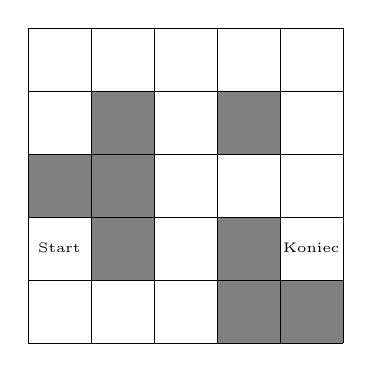
\begin{tikzpicture}[scale=0.8]
        \fill[gray] (1,2) rectangle ++(1,1);
        \fill[gray] (1,3) rectangle ++(1,1);
        \fill[gray] (3,1) rectangle ++(1,1);
        \fill[gray] (3,3) rectangle ++(1,1);
        \fill[gray] (1,1) rectangle ++(1,1);
        \fill[gray] (0,2) rectangle ++(1,1);
        \fill[gray] (3,0) rectangle ++(1,1);
        \fill[gray] (4,0) rectangle ++(1,1);
        
        \node at (0.5,1.5) {\tiny Start};
        \node at (4.5,1.5) {\tiny Koniec};

        \draw[step=1cm,ultra thin,black] (0,0) grid (5,5);
    \end{tikzpicture}
    \caption{\centering Przykładowy labirynt 5x5 z zaznaczonym startem i końcem, gdzie białe pole - przejście, czarne - ściana.}
    \label{fig:example_maze}
\end{figure}